% !TEX program = xelatex
\documentclass[addpoints,12pt]{exam}
\usepackage{fontspec}
\usepackage[T1]{fontenc} % uses T1 fonts (better quality)
\usepackage{lmodern} % uses Latin Modern fonts
% \usepackage[margin=1in]{geometry} % not needed with exam class
\usepackage[dvipsnames]{xcolor}
% \usepackage{ragged2e}
% \renewcommand{\baselinestretch}{1.15}
\usepackage{tikz}
\usetikzlibrary{automata,scopes,shapes,matrix,arrows,decorations.pathmorphing}
\tikzset{>={stealth}}
\usepackage{amsmath,amsfonts,amssymb}
\usepackage{bm}

\usepackage{graphicx}
\graphicspath{ {./graphics/} }
\usepackage{tcolorbox}
\usepackage{etoolbox}
\usepackage[dvipsnames]{xcolor}
\definecolor{CrispBlue}{HTML}{0176AE}

\usepackage[makeroom]{cancel}
\definecolor{OuterBlue}{HTML}{1370AA}
\definecolor{InnerBlue}{HTML}{9BC4DD}
\usepackage{pdfpages}

\BeforeBeginEnvironment{verbatim}{\footnotesize}%
\AfterEndEnvironment{verbatim}{\textnormal}%

\begin{document}
% \setmainfont{SF Pro Text}
% \setsansfont{SF Pro Text}
\setmonofont{SF Mono}
% \renewcommand{\familydefault}{\sfdefault}

\begin{center}
    % \line(1,0){300}\\[0.25cm]
 	\large\bfseries ECE 538 - Advanced Computer Architecture\\[0.5em]
    Homework Assignment 1 (Individual)\\[1em]
    100 points (plus 10 extra credits)\\[1em]
    Assigned Date: \textnormal{09/13/2021} Due Date: \textnormal{09/24/2021}\\[5em]
    David Kirby \quad davidkirby@unm.edu
    \\[5em]
 	% \line(1,0){300}\\[0.75cm]
    \textnormal{
    \cvpword{Credits}\cvbpword{Extra Credits}
    \combinedgradetable[v][questions]}
    \end{center}
    \pagestyle{headandfoot}
    \firstpagefooter{}{\thepage}{}
    \runningfooter{}{\thepage}{}
    \newpage

\begin{questions}
    \pointformat{(\thepoints)}
    \pointpoints{credit}{credits}
    \bonuspointformat{(\thepoints)}
    \bonuspointpoints{extra credit}{extra credits}

\question\textbf{(\pointsofquestion{1} credits)} % Question 1
    For your research, you profiled an application that requires 900 seconds of execution time on a single-core architecture. You would like to design a multi-core architecture to speed up this particular application. Use Amdahl's Law to answer the following questions:
    \begin{parts}
        \part[5] If you were to rewrite the application to take advantage of a multi-core architecture, what would be the maximum achievable speedup on an architecture with four cores? What would the new execution time be? \par
        Assuming 800 seconds of the application’s execution time is perfectly parallelizable, while 100 seconds must be executed sequentially. Also assume the performance of each core in the quad-core architecture equals that of the original single-core architecture.

        \begin{tcolorbox}[colback=CrispBlue!5!white,colframe=CrispBlue!75!black,title=]
        \(  t_{\text{new}} = \frac{800s}{4\text{ cores}} + 100s = 300s\\[1em]
            \text{speedup} = \frac{900s}{300s} = 3\times
        \)
        \end{tcolorbox}
        \vspace{\stretch{1}}

        \part[5] What would be the execution time and speedup achievable with an eight-core machine?

        \begin{tcolorbox}[colback=CrispBlue!5!white,colframe=CrispBlue!75!black,title=]
        \(  t_{\text{new}} = \frac{800s}{8\text{ cores}} + 100s = 200s\\[1em]
            \text{speedup} = \frac{900s}{200s} = 4.5\times
        \)
        \end{tcolorbox}
        \vspace{\stretch{1}}

        \part[5] What would be the maximum speedup achievable on a machine with unlimited cores? 
        
        \begin{tcolorbox}[colback=CrispBlue!5!white,colframe=CrispBlue!75!black,title=]
        \(  t_{\text{new}} = \frac{800s}{\infty\text{ cores}} + 100s = 100s\\[1em]
            \text{speedup} = \frac{900s}{100s} = 9\times
        \)
        \end{tcolorbox}
        \vspace{\stretch{1}}

        \part[5] What would be the maximum speedup achievable on a machine with unlimited cores if 99\% of the execution time could be perfectly parallelized?

        \begin{tcolorbox}[colback=CrispBlue!5!white,colframe=CrispBlue!75!black,title=]
        \(  t_{\text{new}} = \frac{900s \times 0.99}{\infty\text{ cores}} + (900s \times 0.01) = 9s\\[1em]
            \text{speedup} = \frac{900s}{9s} = 100\times
        \)
        \end{tcolorbox}
        \vspace{\stretch{1}}
    \end{parts} 
\newpage 

\question\textbf{(\pointsofquestion{2} credits)} % Question 2
A cryptographic operation takes 1 second to run on a simple embedded processor core. You are considering the design of a coprocessor to accelerate this cryptographic operation in order to improve the energy efficiency of the system. Answer the following questions, using Amdahl's Law where appropriate.
    \begin{parts}
        \part[5] If 95\% of the execution time can be accelerated with a coprocessor, what is the maximum speedup theoretically achievable, assuming no computation overlap between the accelerator and the processor?
        
        \begin{tcolorbox}[colback=CrispBlue!5!white,colframe=CrispBlue!75!black,title=]
            \(  t_{\text{new}} = \frac{1s \times 0.95}{\infty\text{ cores}} + (1s \times 0.05) = 0.05s\\[1em]
                \text{speedup} = \frac{1s}{0.05s} = 20\times
            \)
        \end{tcolorbox}
        \vspace{\stretch{1}}
    
        \part[5] If you were able to design an accelerator that can execute the aforementioned 95\% execution time with a 50x speedup, what would be the maximum achievable speedup of the entire cryptographic operation? What is the new execution time? 
        
        \begin{tcolorbox}[colback=CrispBlue!5!white,colframe=CrispBlue!75!black,title=]
        \(  t_{\text{new}} = \frac{1s \times 0.95}{50\times} + (1s \times 0.05) = 0.069s\\[1em]
            \text{speedup} = \frac{1s}{0.069s} = 14.493\times
        \)
        \end{tcolorbox}
        \vspace{\stretch{1}}

        \part[5] What is the energy improvement of a cryptographic operation with the coprocessor discussed in the previous question if the power of the system doubles with the addition of the accelerator?
        
        \begin{tcolorbox}[colback=CrispBlue!5!white,colframe=CrispBlue!75!black,title=]
        \(  
            \text{Energy improvement} = \frac{\text{old}}{\text{new}} = \frac{14.493\times}{2\times} = 7.246 \times
        \)
        \end{tcolorbox}
        \vspace{\stretch{1}}

        \part[5] Plot the speedup of the overall cryptographic operation as the coprocessor speedup varies from 1x to 50x assuming 95\% of the execution time can be executed on the accelerator. In the same figure, plot the speedup assuming 80\%, 85\%, and 90\% of the execution time can be executed on the accelerator. Be sure to properly label the axis of your graph and use a legend to differentiate between the four different lines. You may use any graphing tool of your choice. \vspace{\stretch{1}} \newpage

        \begin{figure}[ht]
            \centering
            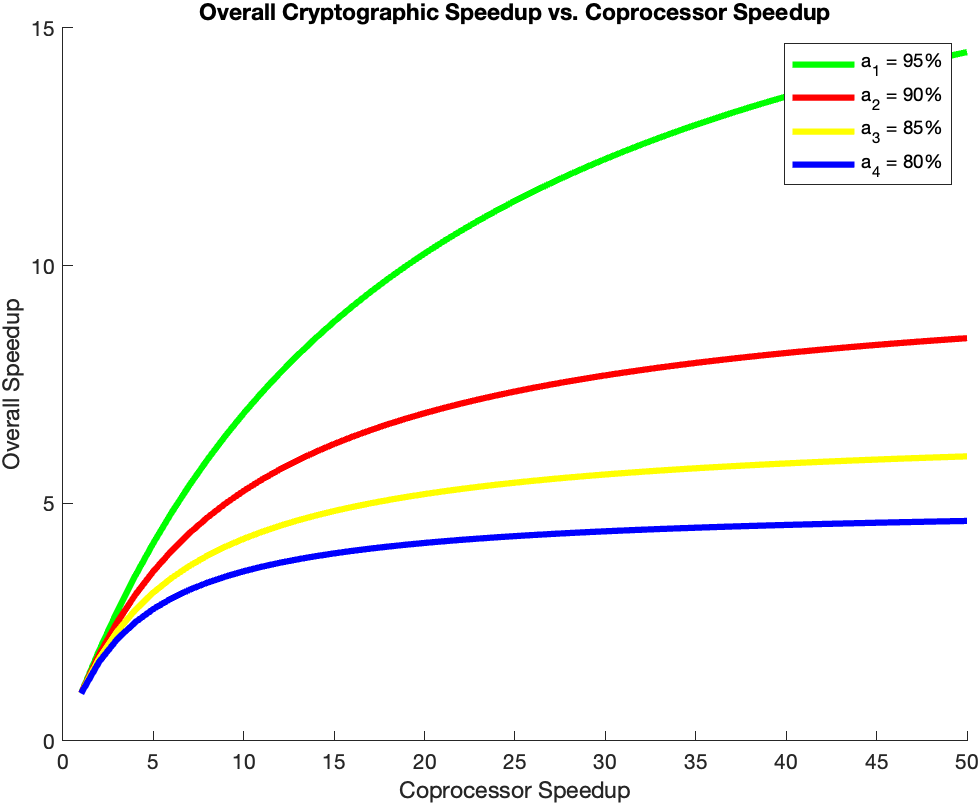
\includegraphics[width=0.85\textwidth]{ECE538-HW01-2d.png}
            \vspace{1em}\caption{Coprocessor Speedup versus Overall Speedup.}
            \label{fig:Coprocessor}
        \end{figure}

        \begin{tcolorbox}[colback=CrispBlue!5!white,colframe=CrispBlue!75!black,title=MATLAB Code]
            \begin{verbatim}
figure(1); clf
coprocessor=1:1:50;
a1=0.95;a2=0.90;a3=0.85;a4=0.80;
overall1=1 ./ ((a1 ./ coprocessor) + (1-a1));
overall2=1 ./ ((a2 ./ coprocessor) + (1-a2));
overall3=1 ./ ((a3 ./ coprocessor) + (1-a3));
overall4=1 ./ ((a4 ./ coprocessor) + (1-a4));
hold
plot(coprocessor,overall1,'g','LineWidth',3)
plot(coprocessor,overall2,'r','LineWidth',3)
plot(coprocessor,overall3,'y','LineWidth',3)
plot(coprocessor,overall4,'b','LineWidth',3)
xlabel('Coprocessor Speedup')
ylabel('Overall Speedup')
title('Overall Cryptographic Speedup vs. Coprocessor Speedup')
legend('a_1 = 95%','a_2 = 90%','a_3 = 85%','a_4 = 80%')\end{verbatim}
        \end{tcolorbox}
    \end{parts}
\newpage 

\question\textbf{(\pointsofquestion{3} credits)} % Question 3
Applications are often times categorized as either computation bound or I/O bound. The former spends most of its execution time on computation, while the latter spends most of its time waiting for I/O (i.e. disk, network access, etc.). The following questions address these differences.
    \begin{parts}
        \part[5] Suppose you have an application that spends 70\% of its time waiting for disk access and 30\% of its time on computation. If you were to run this application on a processor that is 20x faster but with the same I/O speed, what would be the potential speedup?
        
        \begin{tcolorbox}[colback=CrispBlue!5!white,colframe=CrispBlue!75!black,title=]
            \(  t_{\text{new}} = \frac{0.3}{20\times} + 0.7s = 0.715s\\[1em]
            \text{speedup} = \frac{1s}{0.715s} = 1.399\times
            \)
        \end{tcolorbox}
        \vspace{\stretch{1}}

        \part[5] If instead, you ran the application on a system with the same processor speed but a disk that is 2x faster, what would be the potential speedup?
        \begin{tcolorbox}[colback=CrispBlue!5!white,colframe=CrispBlue!75!black,title=]
            \(  t_{\text{new}} = \frac{0.7}{2\times} + 0.3s = 0.65s\\[1em]
            \text{speedup} = \frac{1s}{0.65s} = 1.538\times
            \)
        \end{tcolorbox}
        \vspace{\stretch{1}}
        \part[5] Describe how you might go about improving the disk access of this system.
        \begin{tcolorbox}[colback=CrispBlue!5!white,colframe=CrispBlue!75!black,title=]
            We could improve disk access by using a parallel disk array, by using a flash disk, or by using a disk with higher RPM.
        \end{tcolorbox}
        \vspace{\stretch{1}}
        \part[5] How else might you improve the speed of the overall system in an I/O bound system? How does that compare to that of a computation bound system?
        \begin{tcolorbox}[colback=CrispBlue!5!white,colframe=CrispBlue!75!black,title=]
            I/O bound systems could also be improved by increasing network access (i.e., using an Ethernet connection instead of wireless). The computation bound system was improved by a greater factor simply by increasing disk speed by \(2\times\) compared to \(20\times\) for I/O.
        \end{tcolorbox}
        \vspace{\stretch{1}}
    \end{parts}
\newpage

\question\textbf{(\pointsofquestion{4} credits)} % Question 4
Consider a cluster like the one supported by the Center for Advanced Research Computing (CARC) at UNM. Assume the cluster has 500 computers, each of them with a MTTF of 25 days, and the failures follow an exponential distribution and are independent.
    \begin{parts}
        \part[5] If 1/5 of the computers fail, the cluster is considered to fail. What is the MTTF of the cluster? Under this failure model, does adding more computers increase the MTTF on the cluster? Why?
        \begin{tcolorbox}[colback=CrispBlue!5!white,colframe=CrispBlue!75!black,title=]
            \( \text{MTTF} = \frac{25\text{ days}}{\cancel{500 \text{ computers}}} \times \frac{1}{5} \times \cancel{500} = 5 \text{ days}\\[1em]
            \)
            Under this failure model, MTTF is not dependent on the number of computers and therefore adding more computers would not have an effect on the MTTF of the cluster.
        \end{tcolorbox}
        \vspace{\stretch{1}}
        \part[10] For the same amount of money, one could buy 800 computers, each with MTTF of 20 days. Assume that the cluster (implementation with either 900 less reliable computers or 500 original computers) is considered to fail if a single computer fails. Repairing the less reliable cluster configuration is 10\% less expensive. Which cluster would be better? 
        \begin{tcolorbox}[colback=CrispBlue!5!white,colframe=CrispBlue!75!black,title=]
            \( \text{MTTF} = \frac{20\text{ days}}{800 \text{ computers}} = 0.025 \text{ days or 36 mins}\\[1em]
            \)
            At this rate of failure, even with 10\% savings, it is still \(20\times\) cheaper to go with the more reliable cluster.
        \end{tcolorbox}
        \vspace{\stretch{1}}
        \part[5] If the cluster is considered to fail if a single computer fails, it can be readily shown that adding more computers does not improve MTTF. List reasons why we still would like to have clusters with a larger number of computers (at least three reasons, can be related to reliability, performance and power).
        \begin{tcolorbox}[colback=CrispBlue!5!white,colframe=CrispBlue!75!black,title=]
            Clusters would still allow for parallelized processing, computers could be hot-swapped in and out cutting down on repair times and costs and, due to the parallelized computation, power would be saved.
        \end{tcolorbox}
        \vspace{\stretch{1}}
    \end{parts}
\newpage

\question\textbf{(\pointsofquestion{5} credits)} % Question 5
If you are asked to design the power management (PM) policy for processors used to run a realtime application (e.g., streaming a movie on the mobile device). The application should be completed processing one set of data every 30 milliseconds (ms). The processor contains 4 identical cores: if all cores are at the full speed, the processor consumes 2 Watts (W) (0.5 W for each core); if a core is put into sleep model, the leakage power of the core is 10\% of the dynamic power; If the entire processor is in sleep, the leakage is 15\% of the total dynamic power. Assume that the application is fully parallelizable. \par

Consider three PM policies: 1) Use all 4 cores and run at the full speed. Under this policy, application finishes in 20 ms. 2) Use all 4 cores and run the application by setting the voltage and frequency to 3/4 of what are used at the full speed and then sleep if there is slack time till the deadline. 3) Use 3 cores while letting the \( 4^{th} \) core sleep.
    \begin{parts}
        \part[10] Can policy 2 and 3 meet the deadline requirement of the application? Give the reason.
        \begin{tcolorbox}[colback=CrispBlue!5!white,colframe=CrispBlue!75!black,title=]
            Policy 2: Decreasing the voltage and frequency by 1/4 will result in the time it takes to finish increasing by 1/4 totaling 25 ms.
            
            Policy 3: If 4 cores complete the application in 20 ms, then 3 cores will complete the application in \( \approx \) 26.66 ms.

            Both policy 2 and 3 meet the deadline requirement of the application.
        \end{tcolorbox}
        \vspace{\stretch{1}}
        \part[10] Which option is more energy efficient and why? Which one requires higher peak power (i.e., the maximum power)?
        \begin{tcolorbox}[colback=CrispBlue!5!white,colframe=CrispBlue!75!black,title=]
            Policy 2:\\
            \(\text{Energy} =  \frac{new}{old} = \frac{(\text{Voltage }\times\ 0.75)^2}{\text{Voltage}^2} = 0.5625
            \)\\[1em]
            \( \text{Power}_{\text{dynamic}} = \frac{new}{old} = \frac{0.5625\  \times\ \text{Frequency } \times\ 0.75}{\text{Frequency}} = 0.421875
            \)\\[1em]
            \( \text{Power}_{\text{static}} = 0.421875 \times 15\% = 0.0633
            \)\\[1em]
            \( \text{Power}_{\text{total}} = (0.421875 \times 25 \text{ms}) + (0.0633 \times 5 \text{ms}) = 10.863
            \)\\

            Policy 2 is more energy efficient since changing the voltage has an exponential effect; however, Policy 2 also has a higher peak power due to the execution time burning up more static power.
        \end{tcolorbox}
        \vspace{\stretch{1}}
        \bonuspart[10] Find a policy that leads to the minimum total energy, assuming that no dynamic voltage scaling (i.e., changing the voltage supply level during run time) is allowed. Give the details. \vspace{\stretch{1}}
    \end{parts}
\end{questions}
\end{document}